% Chapter 3

\chapter{Πειραματική Διάταξη και Συγκριτική αξιολόγηση} % Main chapter title

\label{Chapter3} % For referencing the chapter elsewhere, use \ref{Chapter3} 
%----------------------------------------------------------------------------------------

% Define some commands to keep the formatting separated from the content 


%----------------------------------------------------------------------------------------

\section{Γενικά}

Σκοπός αυτού του κεφαλαίου είναι να πραγματοποιηθεί μία συστηματική αξιολόγηση των αλγορίθμων που παρουσιάστηκαν στο προηγούμενο κεφάλαιο, σε σχέση με το σύστημα \emph{Auto-TSAD}, κάτω από ένα τυποποιημένο πρότυπο αναφοράς, όπως το \emph{TSB-UAD}.

Τα δεδομένα τα οποία χρησιμοποιήθηκαν για την εκτέλεση των πειραμάτων ήταν από 2 datasets τα οποία είχαν συλλεχτεί από τους δημιουργούς του \emph{TSB-UAD}, το \emph{public\_v2} το οποίο υπάρχει διαθέσιμο στο \href{https://www.thedatum.org/datasets/TSB-UAD-Public-v2.zip}{public\_v2 dataset} καθώς και το \emph{Artificial dataset} το οποίο είναι διαθέσιμο στο \href{https://www.thedatum.org/datasets/TSB-UAD-Artificial.zip}{artificial dataset}. 

Για κάθε dataset έγιναν 2 διαφορετικά πειράματα στο \emph{Auto\_TSAD}, ένα με ενεργοποιημένη την μηχανή βελτιστοποίησης \emph{optuna}, η οποία απαιτούσε αρκετό χρόνο για να εκτελέσει ένα πείραμα, και ένα με κλειστή την μηχανή βελτιστοποίησης. Έτσι o αριθμός των χρονοσειρών που εκτελέστηκαν σε κάθε πείραμα, έχουν όπως στον πίνακα \ref{tab:experiments_num}:

\begin{table}[h]
\centering
\caption{Experiments For Auto-TSAD with/out for each dataset}
\label{tab:experiments_num}
\begin{tabular}{lcc}
\toprule
Dataset & Optuna-ON & Optuna-OFF \\
\midrule
Public V2 & 29 & 3429 \\
Artificial & 236 & 960 \\
\bottomrule
\end{tabular}
\end{table}
\subsection{Μετρικές Αξιολόγησης}
Οι μετρικές που αξιολογήθηκαν ήταν ο χρόνος που απαιτήθηκε, καθώς και το score που πέτυχε η κάθε τεχνική με βάση την μετρική \strong{VUS-ROC}. O χρόνος σε συνάρτηση με την \emph{ROC-VUS} είναι σημαντικά, καθώς μας επιτρέπει να αξιολογήσουμε αν η διαφορά στον εντοπισμό των ανωμαλιών είναι αρκετά μεγάλη, για να δικαιολογήσει και το χρονικό κόστος που απαιτεί η μηχανή βελτιστοποίησης \emph{optuna} του \emph{Auto-TSAD}.

\subsection{Γενικές Παρατηρήσεις}
Σαν μία γενική πρώτη παρατήρηση είναι πως το \emph{Auto-TSAD} δεν μπορεί να αποδόσει σωστά χωρίς να έχουμε ενεργοποιήσει την \emph{optuna}. Συγκεκριμένα, το ποσοστό επιτυχίας του, ώστε να μπορέσει να βρει έστω και μία ανωμαλία, ήταν πολυ χαμηλό όταν δεν ήταν ενεργοποιημένη η \emph{optuna}. Τα αποτελέσματα φαίνονται στο Σχήμα \ref{figure:success_rates_tsad}. Παρατηρούμε τόσο στο \emph{Public} όσο και στο \emph{Artificial} dataset, το ποσοστό επιτυχίας ανίχνευσης έστω και μίας ανωμαλίας αγγίζει το $100\%$ όταν η \emph{optuna} είναι ενεργοποιημένη, ενώ αντιθέτως τα ποσοστά επιτυχίας είναι πολύ πιο χαμηλά με τιμές $31,2\%$ για το \emph{Public} και $9,2\%$ για το \emph{Artificial} dataset.
Συγκεκριμένα, χωρίς την \emph{optuna} ενεργοποιημένη, το σύστημα \emph{Auto-TSAD} δεν μπόρεσε να πάραξει κανένα αποτέλεσμα, για καμία μετρική. Το σύστημα \emph{Auto-TSAD} υπολογίζει την απόδοση στις παρακάτω μετρικές:

\begin{itemize}
    \item PrAUC
    \item RocAUC
    \item RangePrAUC
    \item RangeRocAUC
    \item RangePrVUS
    \item RangeRocVUS
    \item RangePrecision
    \item RangeRecall
    \item RangeFScore
    \item Precision
    \item Recall
    \item FScore
    \item PrecisionAtK
\end{itemize}

\begin{figure}[h]
    \centering
    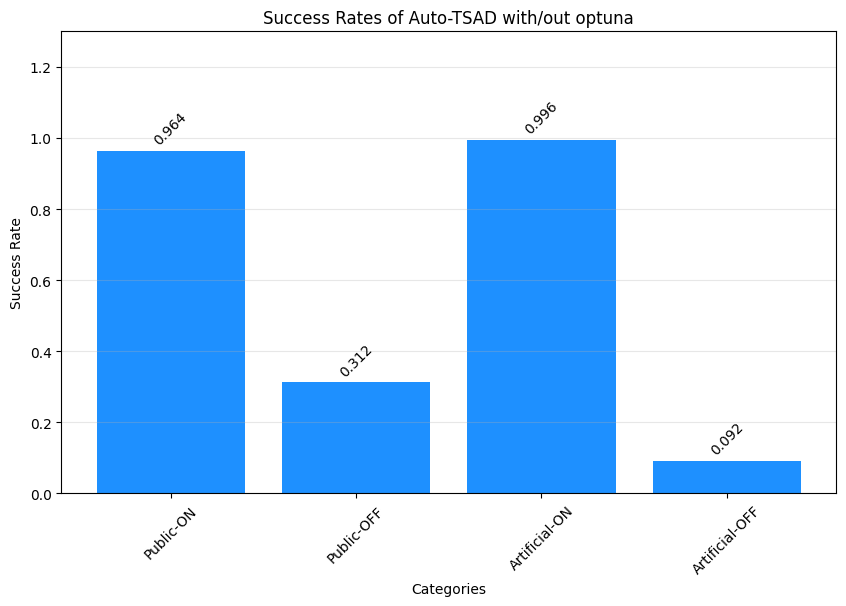
\includegraphics[width=1\linewidth]{Figures/success_rates_tsad.png}
    \caption{Ποσοστά επιτυχίας ανίχνευσης τουλάχιστον μίας ανωμαλίας του Auto-TSAD}
    \label{figure:success_rates_tsad}
\end{figure}

\subsection{TODO}
\textcolor{red}{TODO ΓΙΑΤΙ ΔΕΝ ΕΠΙΣΤΡΕΦΕΙ ΟΜΩΣ ΑΠΟΤΕΛΕΣΜΑΤΑ? ΔΕΝ ΕΙΝΑΙ ΠΕΡΙΟΔΙΚΑ??}
 
\section{Public Dataset}
Σε αυτό το κεφάλαιο θα συγκρίνουμε τα αποτελέσματα του \emph{Auto-TSAD} με τις άλλες μετρικές \emph{IForesit - POLY - MP}.
Για το \emph{Auto-TSAD}, με ανοιχτή την μηχανή βελτιστοποίησης \emph{optuna}, επιλέχτηκε τυχαία μία χρονοσειρά από κάθε dataset, ενώ με κλειστή την μηχανή \emph{optuna}, ο \emph{Auto-TSAD} έτρεξε στο σύνολο των χρονοσειρών. Οι μετρικές \emph{IForest - POLY - MP} εκτελέστηκαν μόνο στις ίδιες επιλεγμένες χρονοσειρές που έτρεξε και ο \emph{Auto-TSAD}.

\subsection{Τα dataset}
Τα dataset που επιλέχτηκαν από τους δημιουργούς του \emph{Auto-TSAD}, καλύπτουν μία ευρεία γκάμα από διαφορετικούς τομείς, με διαφορετικούς τύπους ανωμαλιών. Πιο συγκεκριμένα:
\begin{itemize}
    \item \emph{Genesis}: Προέρχεται από έναν φορητό επιδείτη τοποθέτησης και μεταφοράς, ο οποίος χρησιμοποιεί μία δεξανμενή αέρα για να τροφοδοήσει ρομποτικές μονάδες λαβής και αποθήκευσης. Περιέχει ακολουθίες ανωμαλιών.
    \item \emph{WSD}: Αφορά χρονοσειρές που συλλέγουν δεδομένα από μεγάλες εταιρίες του Διαδικτύου, και περιέχουν Βασικούς Δείκτες Απόδοσης. Περιέχει ακολουθίες ανωμαλιών.
    \item \emph{MSL}: Συλλογή δεδομένων της NASA που προέρχονται από τους αισθητήρες του Rover Curiosity από τον Άρη. Περιέχει ακολουθίες ανωμαλιών.
    \item \emph{Stock}: Αφορά δεδομένα από αγορές μετοχών.Περιέχει ανωμαλές σημείων.
    \item \emph{Dapnhet}: Ιατρικά δεδομένα που σχετίζονται με την νόσο του Parkinson. Καταγράφει ενδείξεις από 3 αισθητήρες επιτάχυνσης οι οποίοι είναι τοποθετημένοι στο ισχύο και στο πόδι ασθενών, και εντοπίζουν το φαινόμενο freezing of gate (FoG) κατά τη διάρκεια εργασιών περπατήματος. Περιέχει ακολουθίες ανωμαλιών.
    \item \emph{MITDB}: Αφορά δεδομένα που συλλέχτηκαν από 47 ασθενής, και περιέχει 48 αποσπάσματα μισής ώρας ηλεκτροκαρδιογραφημάτων διπλού καναλιού, και προσπαθούν να εντοπίσουν καρδιακές αρυθμίες. Περιέχει ακολουθίες ανωμαλιών.
    \item \emph{GHL}: Αφορά δεδομένα τα οποία συλλέγονται από 3 δεξαμενές σε έναν βρόγχο θέρμανσης πετρελαίου. Καταγράφει την θερμοκρασία και την στάθμη τους. Οι ανωμαλίες αντιστοιχούν σε αλλαγές στην μέγιστη θερμοκρασία ή την συχνότητα της αντλίας. Πρόκειται για ακολουθίες ανωμαλιών.
    \item \emph{Sensorscope}: Μία συλλογή από περιβαλλοντικά δεδομένα που αφορούν θερμοκρασία, υγρασία, ηλιακή ακτινοβολία κ.ο.κ. Πρόκειται για ακολουθίες ανωμαλιών.
    \item \emph{SMD}: Δεδομένα καταγραφής λειτουργίας 28 διαφορετικών server, 3 διαφορετικών ομάδων, διάρκειας 5 εβδομάδων από μεγάλη εταιρία Διαδικτύου. Περιέχει ακολουθίες ανωμαλιών.
    \item \emph{MGAB}: Αποτελείται από χρονοσειρές Mackey-Grass, η οποίες παρουσιάζουν χαοτική συμπεριφορά, κάνοντας πολύ δύσκολο το έργο ανίχνευσης ανωμαλιών με γυμνό μάτι. Περιέχει ακολουθίες ανωμαλιών.
    \item \emph{NAB}: Σύνθετα δεδομένα από πραγματικές και τενητές χρονοσειρές, οι οποίες προέρχονται από διάφορους server, όπως AWS, αναφορές στο \emph{X} σε μεγάλες εισηγμένες εταιρίες κ.ο.κ. Περιλαμβάνει ακολουθίες ανωμαλιών.
    \item \emph{SED}: Αφορά δεδομένα από δίσκους κινητήρων της NASA σε διάφορες φάσης λειτουργίας, σε σταθέ ταχύτητα $3000 rpm$. Αφορά ακολουθίες ανωμαλιών.
    \item \emph{SVDBM}: Περιλαμβάνει 78 ιατρικά καρδιογραφήματα, ημίωρης διάρκειας, επιλεγμένες ειδικά για να συμπληρώσουν το \emph{MITB}. Περιέχει ακολουθίες ανωμαλιών.
    \item \emph{Dodgers}: Δεδομένα καταγραφής κίνησης στον αυτοκινητόδρομο 101 του LA, μετά το τέλος αγώνα της ομάδας μπέιζμπολ Dodgers. Περιέχει ακολουθίες ανωμαλιών.
    \item \emph{TAO}: Δεδομένα που αφορούν μετεωρολογικές και ωκεανογραφικές μετρήσεις. Περιέχει και μεμονωμένες ανωμαλίες αλλά και ακολουθίες ανωμαλιών.
    \item \emph{IOPS}: Δεδομένα που αφορούν την ποιότητα των διαδικτυακών υπηρεσιών και την υγεία ενός μηχανήματος. Περιέχει ακολουθίες ανωμαλιών.
    \item \emph{OPPORTUNITY}: Αφορά αισθητήρες οι οποίοι συλλέγουν δεδομένα κατά την ανθρώπινη δραστηριότητα. Περιέχει ακολουθίες ανωμαλιών.
    \item \emph{NEK}: Περίεει δεδομένα από διαδικτυακές συσκευές παραγωγής. Περιέχει τόσο σημειακές ανωμαλίες όσο και ακολυθίες ανωμαλιών.
    \item \emph{CreditCard}: Αφορά δεδομένα συναλλαγών μέσω πιστωτικών καρτών. Προσπαθεί να εντοπίσει απάτες. Περιέχει μεμονωμένες ανωμαλίες καθώς και ακολουθίες ανωμαλιών.
    \item \emph{CATSv2}: Περιλαμβάνει δεδομένα από εντολές συστήματος, εξωτερικά ερεθίσματα και μετρήσεις τηλεμετρίας, στις οποίες έχουν εισαχθεί 200 ανωμαλίες. Περιέχει ακολουθίες ανωμαλιών.
    \item \emph{TODS}: Συνθετικό dataset το οποίο περιέχει διαφορετικού τύπου δεδομένων για την αξιολόγηση αλγορίθμων εύρεσης ανωμαλιών. Περιέχει τόσο μεμονωμένες ανωμαλίες καθώς και ακολουθίες ανωμαλιών.
    \item \emph{Power}: Καταγράφει δεδομένα ζήτησης/κατανάλωσης ενέργειας. Περιέχει ακολουθίες ανωμαλιών.
    \item \emph{UCR}: Συλλογή από διάφορες μονοσδιάστατες χρονοσειρές, από διάφορους τομείς, στις οποίες οι περισσότερες ανωμαλίες έχουν εισηχθή τεχνητά. Περιέχει και μεμονωμένες ανωμαλίες αλλά και ακολυθίες ανωμαλιών.
    \item \emph{SMAP}: Πραγματικά δεδομένα από καταγραφές και μετρήσεις αεροδιαστημικών συστημάτων και δορυφόρων. Περιέχει ακολουθίες ανωμαλιών.
    \item \emph{SWaT}: Περιλαμβάνει δεδομένα τα οποία προέρχονται από 51 ασθητήρες και ενεργοποιητές, όπου αναλύουν το νερό. Οι ανωμαλίες αντιπροσωπεύουν λάθος ενδείξεις στις μετρήσεις των αισθητήρων λόγο κυβερνοεπιθέσεων. Περιέχει ακολουθίες ανωμαλιών.
    \item \emph{YAHOO}: Περιλαμβάνει δεδομένα τα οποία προέρχονται από τα εργαστήρια της YAHOO και αφορά πραγματικές και συνθετικές χρονοσειρές, βασισμένες στην πραγματική κίνηση παραγωγής διάφορων συστημάτων της εταιρίας. Περιέχει τόσο μεμονωμένες ανωμαλίες, αλλά και ακολουθίες ανωμαλιών.
    \item \emph{GECCO}: Dataset το οποίο αφορά στην ποιότητα του νερού, για online ανίχνευση ανωμαλιών. Περιέχει ακολουθίες ανωμαλιών.
    \item \emph{EXATHLON}: Δεδομένα από πραγματικα ίχνη δεδομένων, τα οποία συλλέχτηκαν επί 2,5 μήνες από ένα Spark cluster. Για κάθε ανωμαλία παρέχονται ακριβές ετικέτες τόσο για το χρονικό διάστημα της βασικής αιτίας, αλλά και για το χρονικό διάστημα των επιπτώσεων. Περιέχει ακολουθίες ανωμαλιών.
\end{itemize}
\subsection{Χρόνοι εκτέλεσης}
Τα πειράματα εκτελέστηκαν σε τρία μηχανήματα με λειτουργικό σύστημα Fedora Linux 43. Το πρώτο μηχάνημα διέθετε επεξεργαστή Intel Core i5-10400 (6 πυρήνες, 4GHz), κάρτα γραφικών AMD Radeon RX 5700 XT και 16GB μνήμης RAM DDR4. Τα υπόλοιπα δύο μηχανήματα ήταν ίδια μεταξύ τους, με επεξεργαστή Intel Core i5-9500T (6 πυρήνες, 2.2GHz), ενσωματωμένη κάρτα γραφικών Intel UHD Graphics 630 και 16GB μνήμης RAM DDR4.

Όπως αναφέρθηκε και προηγουμένως, σημαντικό είναι να εξετάσουμε τους χρόνους εκτέλεσης. Η μηχανής βελτιστοποίησης της \emph{optuna}, που χρησιμοποιεί το \emph{Auto-TSAD} απαιτεί αρκετό χρόνο για να υπολογίσει και να βρει τις καλύτερες υπερπαράμετρους για τον κάθε αλγόριθμο, ώστε να καταλήξει στην χρήση ενός αλγόριθμου με τις καλύτερες δυνατές υπερπαραμέτρους. Τα αποτελέσματα φαίνονται συγκεντρωτικά στο Σχήμα \ref{figure:time_optuna_on}. Ο μέγιστος χρόνος εκτέλεσης που παρατηρήθηκε, ήταν 37,1 ώρες (37 ώρες και 6 λεπτά) για το dataset \emph{TAO}, ενώ ο ελάχιστος χρόνος ήταν 0,4 ώρες (24 λετπά). Επίσης η μέση τιμή είναι 3,84 ώρες (3 ώρες και 50 λεπτά) και η τυπική απόκλιση είναι 7,35 ώρες (7 ώρες και 21 λεπτά). Συγκεντρωτικά όλα τα στατιστικά στοιχεία φαίνονται στον πίνακα.

\begin{figure}[h]
    \centering
    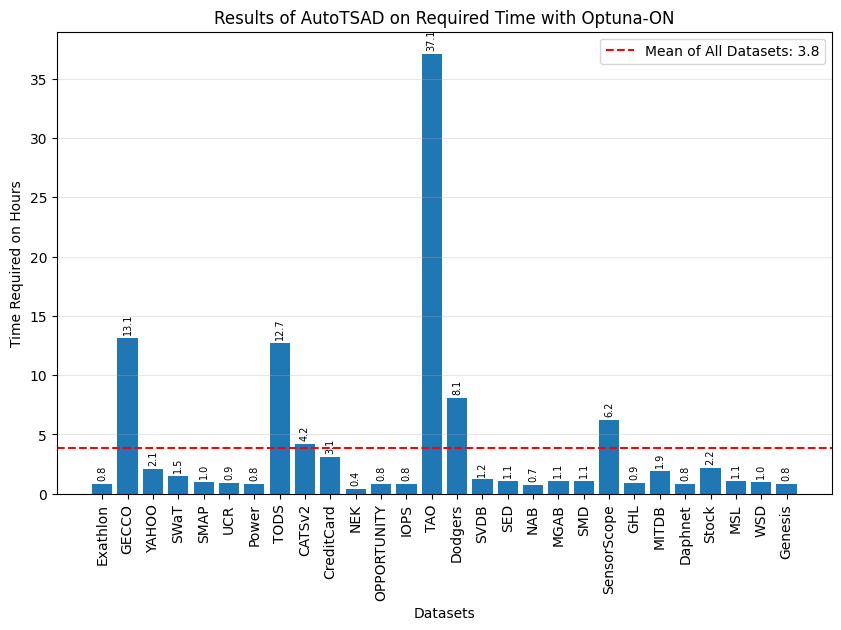
\includegraphics[width=1\linewidth]{Figures/v2_time_optuna-on_tsad.png}
    \caption{Χρόνοι εκτέλεσης για κάθε dataset με ανοιχτή την μηχανή βελτιστοποίησης optuna, σε ώρες.}
    \label{figure:time_optuna_on}
\end{figure}

\begin{table}[h]
\centering
\caption{Στατιστικά χρόνου εκτέλεσης με την optuna στο publicv2 dataset}
\label{tab:statistics-optuna-on}
\begin{tabular}{lc}
\toprule
Measure & Value \\
\midrule
Mean & 3.84  \\
std & 7.35 \\
min & 0.40 \\
25\% & 0.80 \\
50\% & 1.10 \\
75\% & 2.43 \\
max & 37.10\\ 
\bottomrule
\end{tabular}
\end{table}

Ενώ το 75\% των dataset εκτελούντε μέχρι 2 ώρες και 26 λεπτά, υπάρχουν και κάποια dataset όπως το \emph{GECCO, TODS, TAO, DODGERS και SensorScope} για τα οποία απαιτήθηκε πολύ παραπάνω χρόνος εκτέλεσης. Αυτά τα δεδομένα, δεν παρουσιάζουν όλα μαζί κάποιο ενιαίο χαρακτηριστικό, το οποίο να δικαιολογεί συνολικά τον τόσο αυξημένο χρόνο εκτέλεσής του. Παρ' όλα αυτά, μία πιθανή εξήγηση είναι η εξής:
\begin{itemize}
    \item To \emph{GECCO} και το \emph{DODGERS} έχουν σαν μέσο μήκος χρονοσειράς, 138.000 και 50.400 σημεία αντίστοιχα. Το \emph{Auto-TSAD} επειδή μπορεί να εκτελέσει τον κάθε αλγόριθμο μέχρι και 800 φορές για την εύρεση των καλύτερων υπερπαραμέτρων, σε συνδιασμό με τον μεγάλο όγκο των δεδομένων, μπορεί να εκτοξεύσει τους χρόνους εκτέλεσης.
    \item Το \emph{TAO} και το \emph{TODS}, ενώ δεν έχουν τόσο μεγάλο μήκος χρονοσειρών, φαίνεται ότι έχουν σχετικά υψηλό ποσοστό ανωμαλιών, με 9,4\% και 6,3\% αντιστοίχως, καθώς επίσης οι τύποι των ανωμαλιών που περιέχουν είναι και μεμονωμένες ανωμαλίες αλλά και ακολουθίες ανωμαλιών.
    \item Τέλος το \emph{SensorScope} αλλά και το \emph{DODGERS} παρουσιάζουν πολύ υψηλό ποσοστό ανωμαλιών με 22,5\% και 11,14\% αντίστοιχα.
\end{itemize}
Γενικά, φαίνεται πως αλγόριθμοι οι οποίοι δεν μπορούν να κλιμακώσουν σωστά σε μεγάλο σετ δεδομένων, ή με πολλές ανωμαλίες, δυσκολεύουν πάρα πολύ την μηχανή της Optuna και πολλές φορές αναγκάζεται να τρέξει σχεδόν όλες τις επαναλήψεις για όλους τους αλγορίθμους που χρησιμοποποιεί, καθώς δεν μπορεί να βρει 10 σετ υπερπαραμέτρων με απόδοση μεγαλύτερη του 95\% για να σταματήσει την λειτουργία της. 

Οι χρόνοι εκτέλεσης χωρίς ανοιχτή την μηχανή \emph{Optuna} είναι πολύ μικρότεροι, με μέσο χρόνο εκτέλεσης τα 3 λεπτά και τυπική απόκλιση 12 λεπτών. Ενδιαφέρον εύρημα αποτελεί ο μέγιστος χρόνος εκτέλεσης, ο οποίος ανέρχεται σε 6 ώρες και 41 λεπτά, o οποίος ανήκει στην χρονοσειρά με όνομα LTDB\textbackslash14157\_col\_0 η οποία βρέθηκε να έχει $9.5 \times 10^{6}$ σημεία. Τα αποτελέσματα βρίσκονται στον πίνακα \ref{optuna-off_runtime_pv2_with_outlier}. Αν επαναυπολογήσουμε τα καινούργια στατιστικά, χωρίς αυήν την ακράια τιμή, τότε η καινούργια μέση τιμή έιναι ίση με 167 sec, ενώ η καινούργια τυπική απόκλιση είναι 74 sec, όπως φαίνεται και στον πίνακα \ref{optuna-off_runtime_pv2_without_outlier}.
\begin{table}[h]
    \centering
    \caption{Χρόνοι εκτέλεσης σε sec στο dataset public v2, χωρίς ενεργή την μηχανή βελτιστοποίησης}
    \label{optuna-off_runtime_pv2_with_outlier} 
    \begin{tabular}{lc}
        \toprule
        Statistics & Runtimes in seconds \\
        \midrule
            mean & 190 \\
            std & 736 \\
            median & 54 \\
            min & 3 \\
            max & 24109 \\
        \bottomrule
    \end{tabular}
\end{table}

\begin{table}
    \centering
    \caption{Χρόνοι εκτέλεσης σε sec στο dataset public v2, χωρίς ενεργή την μηχανή βελτιστοποίησης και χωρίς ακραίες τιμές}
    \label{optuna-off_runtime_pv2_without_outlier} 
    \begin{tabular}{lc}
        \toprule
        Statistics & Runtimes in seconds \\
        \midrule
            mean & 167 \\
            std & 74 \\
        \bottomrule
    \end{tabular}
\end{table}

Όσον αφορά το \emph{TSB-UAD}, εξετάστηκαν οι χρόνοι εκτέλεσης των αλγορίθμων \emph{IForest - POLY} και \emph{MP}, καθώς δεν υπήρχε πρόσβαση στον αλγόριθμο \emph{NORMA} από τους δημιουργούς του \emph{TSB-UAD}. Η εφαρμογή τους έγινε πάνω στις ίδιες χρονοσειρές οι οποίες επιλέχτηκαν από το \emph{Auto-TSAD} με ενεργοποιημένη την μηχανή \emph{Optuna} για να βγουν όσο το δυνατό πιο αντικειμενικά αποτελέσματα. Ο υπολογισμός του χρόνου για κάθε αλγόριθμο, αφορά από την εκπαίδευση των μοντέλων μέχρι και την εξαγωγή των score, ενώ δεν συμπεριλήφθηκε ο υπολογισμός των μετρικών.Για την ανάπτυξη του κώδικα, χρησιμοποιήθηκε το notebook το οποίο υπάρχει στο github repository των δημιουργών του \emph{TSB-UAD}, το οποίο βρίσκεται στον σύνδεσμο \href{https://github.com/TheDatumOrg/TSB-UAD/blob/main/example/notebooks/test_anomaly_detectors.ipynb}{Anomaly detection for time series from TSB-UAD authors}. Ο κώδικας για την εκτέλεση των τριών αλγορίθμων έχει όπως στα Σχήματα \ref{figure:runIforest} έως \ref{figure:runMP}. TODO ΜΑΛΛΟΝ ΠΡΕΠΕΙ ΝΑ ΓΡΑΨΩ ΚΑΙ ΤΙ ΚΑΝΕΙ Ο ΚΩΔΙΚΑΣ ΕΔΩ !!!!!!!!!!!!!!!!!!!!!!   

\begin{figure}[h]
    \centering
    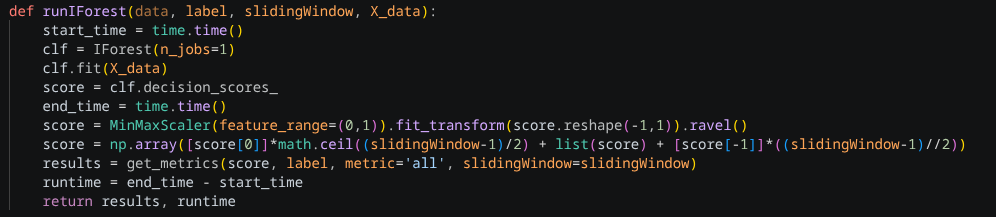
\includegraphics[width=1\linewidth]{Figures/run_IForest.png}
    \caption{Κώδικας για την εκτέλεση του IForest μέσω του TSB-UAD}
    \label{figure:runIforest}
\end{figure}

\begin{figure}[h]
    \centering
    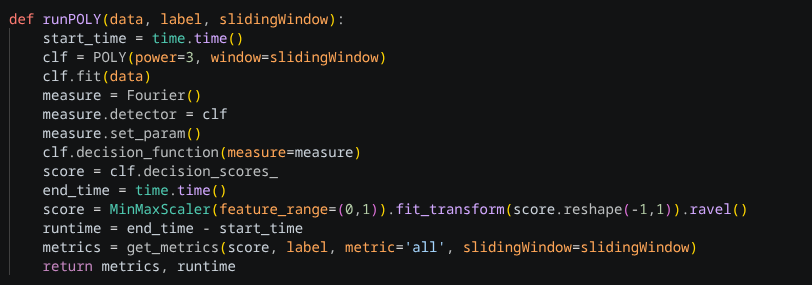
\includegraphics[width=1\linewidth]{Figures/runPOLY.png}
    \caption{Κώδικας για την εκτέλεση του POLY μέσω του TSB-UAD}
    \label{figure:runPOLY}
\end{figure}

\begin{figure}[h]
    \centering
    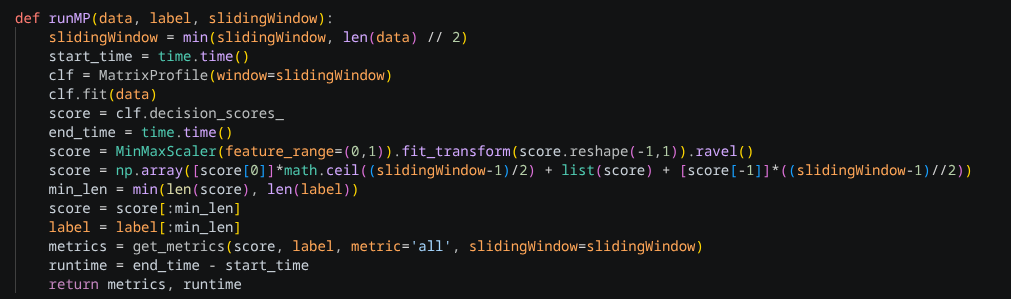
\includegraphics[width=1\linewidth]{Figures/runMP.png}
    \caption{Κώδικας για την εκτέλεση του MP μέσω του TSB-UAD}
    \label{figure:runMP}
\end{figure}

Οι απαιτήσεις εκτέλεσης αυτών των αλγορίθμων ήταν πολύ μικρές, της τάξης των 5-6 δευτερολέπτων μέγιστο για τους \emph{IForest} και \emph{POLY}, ενώ για τον \emph{MP} κάποιες φορές απαιτήθηκε παραπάνω χρόνος, με μέγιστες τιμές μέχρι και 800 δευτερόλεπτα. Σαν γενική εντύπωση είναι πως το \emph{TSB-UAD} χρειάστηκε αρκετά μικρότερο χρόνο (της τάξης των δευτερολέπτων μέχρι και κάποιων λεπτών) σε αντίθεση με το \emph{Auto-TSAD} το οποίο σε εξαιρετικές περιπτώσεις απαιτούσε ακόμα και μέρες για να παράξει αποτελέσματα. Στο σχήμα \ref{figure:tsb-times} παρουσιάζονται οι χρονικές απαιτήσεις του κάθε αλγορίθμου που εκτελέστηκαν μέσω του \emph{TSB-UAD}. Παρότι οι αλγόριθμοι που έτρεχαν στο \emph{TSB-UAD} απαιτούσαν σχεδόν μηδενικό χρόνο σε σύγκριση με \emph{Auto-TSAD}, είναι σημαντικό πως, όπως θα δούμε παρακάτω, όλοι κατάφεραν να παράξουν αποτελέσματα, δηλαδή να ανιχνέυσουν ανωμαλίες (το ποσοστό αποτυχίας ανίχνευσης ανωμαλιών του \emph{Auto-TSAD} με κλειστή την μηχανή της Optuna ήταν $\approx 69\%$).

\begin{figure}[h]
    \centering
    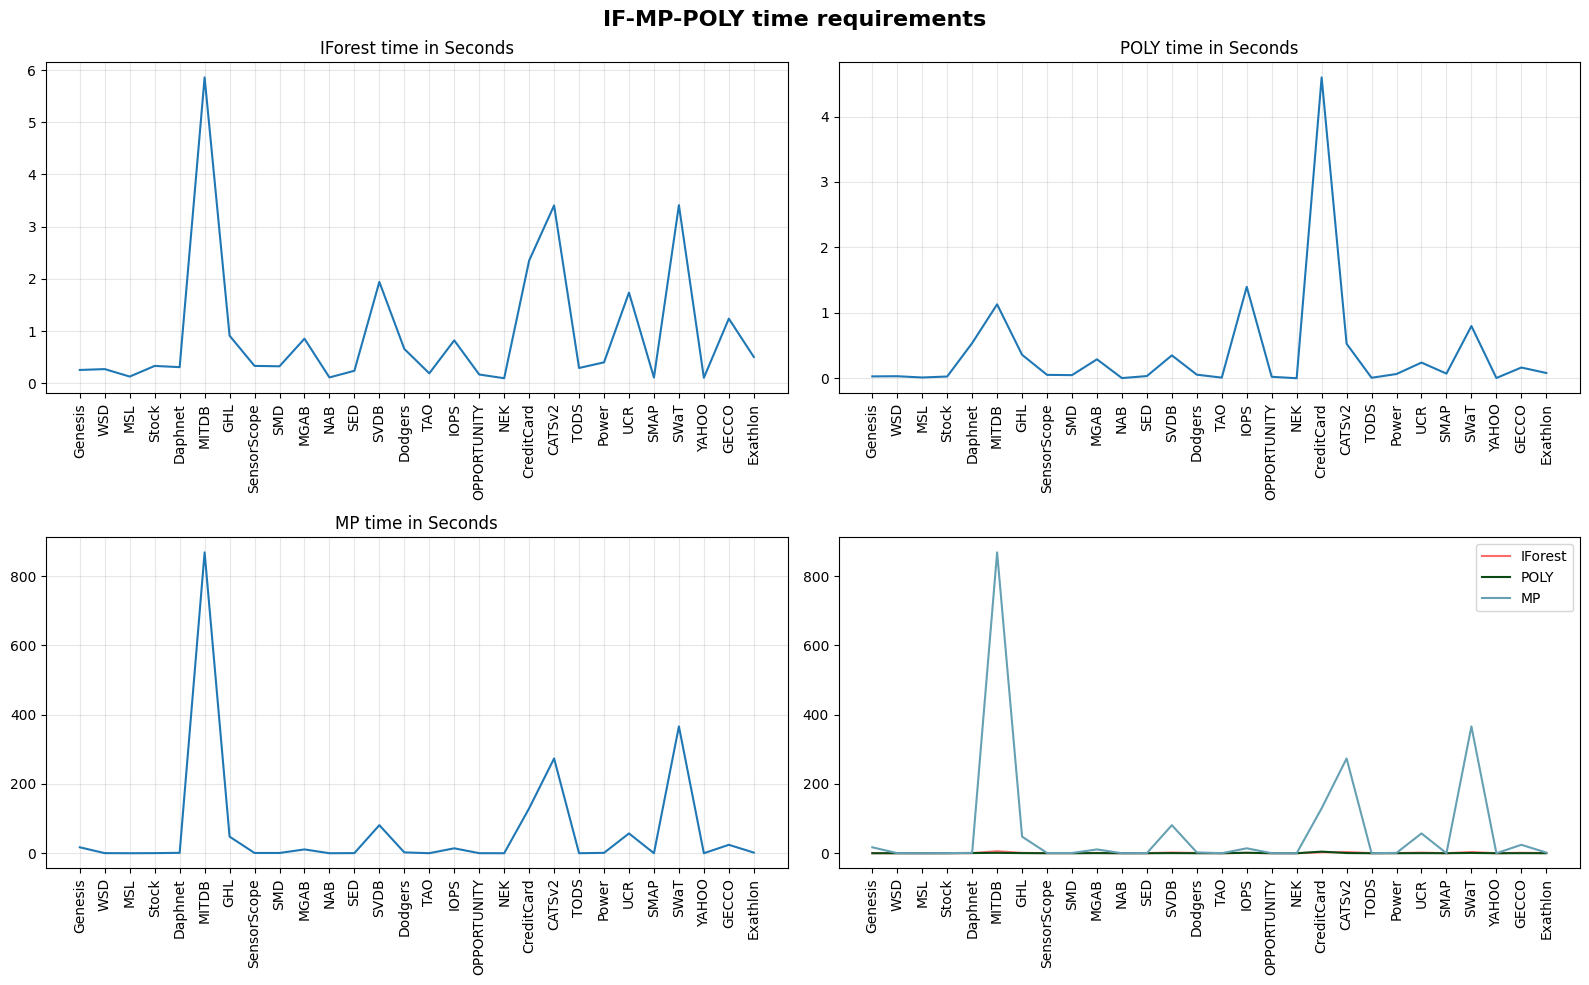
\includegraphics[width=1\linewidth]{Figures/v2_time_tsb.png}
    \caption{Κώδικας για την εκτέλεση του MP μέσω του TSB-UAD. 
        Πάνω αριστερά διακρίνουμε τις χρονικές απαιτήσεις του IForest. 
        Πάνω δεξιά της χρονικές απαιτήσεις του POLY. 
        Κάτω αριστερά διακρίνουμε τις χρονικές απαιτήσεις του MP. 
        Κάτω δεξιά διακρίνουμε συγκριτικά τις χρονικές απαιτήσεις όλων των αλγόριθμων.}
    \label{figure:tsb-times}
\end{figure}

\subsection{Αποτελέσματα ROC-VUS}
Θα εξετάσουμε τα αποτελέσματα της μετρικής \emph{ROC-VUS}:
\begin{enumerate}
    \item Mε ανοιχτή την Optuna και μεταξύ των αλγορίθμων που τρέχουμε στο \emph{TSB-UAD}
    \item Με κλειστή την Optuna και μεταξύ των αλγορίθμων που τρέχουμε στο \emph{TSB-UAD}
    \item Μεταξύ όλων των αποτελεσμάτων
\end{enumerate}
Έτσι θα έχουμε μία πιο σφαιρική άποψη για την επίδραση της Optuna στην εύρεση των ανωμαλιών.
\subsubsection{Συγκριτικά αποτελέσματα με Optuna-ON}

Τα αποτελέσματα της χρήσης της μηχανής της Optuna, είναι, όπως φαίνεται και στο Σχήμα \ref{figure:tsad-vus-on}, αρκετά εντυπωσιακά. Στα περισσότερα dataset, ανακάλυψε επιτυχημένα πάνω από το $90\%$ των ανωμαλιών, ενώ σημαντικό είναι επίσης το γεγονός, πως σε αρκετά το ποσοστό επιτυχίας ήταν $\geq 99\%$. O μέσος όρος των αποτελεσμάτων ήταν $87,13\%$, ενώ στα dataset \emph{NAB, MITDB, CATSv2}, δεν πέτυχε υψηλά ποσοστά επιτυχίας, καθώς επίσης και στο dataset \emph{NEK} δεν μπόρεσε να βρεί καμία ανωμαλία, παρόλο που χρειάστηκε να δαπανηθούν 24 λεπτά για την εύρεση υπερπαραμέτρων. Από ότι φαίνεται από τα log files της εκτέλεσης, δεν μπόρεσε να βρεθεί κάποια περίοδος, τα δεδομένα εκπαίδευσης παράχτηκαν στα τυφλά, με αποτέλεσμα κατά την φάση της αποκοπής των αλγορίθμων, να επηζήσουν μόνο 2 διαφορετικές εκτελέσης του αλγορίθμου \emph{STOMP}, η μία μάλιστα με default παραμέτρους anomaly window size = 10, εκ των οποίων κανείς δεν μπορεί να παράξει αποτελέσματα. 

\begin{figure}[h]
    \centering
    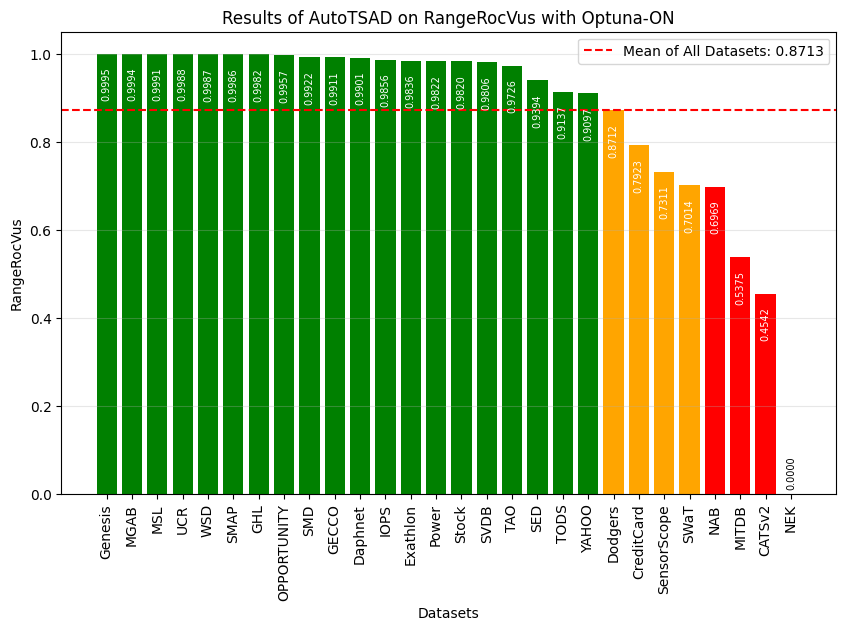
\includegraphics[width=1\linewidth]{Figures/v2_optuna-on_VUS.png}
    \caption{Συγκριτικά αποτελέσματα αλγορίθμων IForest - POLY - MP στην μετρική ROC-VUS.}
    \label{figure:tsad-vus-on}
\end{figure}

Από τους αλγορίθμους που εκτελέστηκαν από το \emph{TSB-UAD}, μπορούμε στο σχήμα \ref{figure:tsad-vus-compare} να παρατηρήσουμε την απόδοσή τους σε κάθε dataset μεμονωμένα, όπως επίσης και συγκριτικά πως τα πήγαν όλοι μαζί. Στο πάνω αριστερά σχήμα βλέπουμε την απόδοση του \emph{Iforest}, ο οποίοις φαίνεται ότι στα περισσότερα αποτελέσματα πέτυχε μία ικανοποιητική ανίχνευση ανωμαλιών, με χαμηλότερα αποτελέσματα να έχει πετύχει στα dataset \emph{WSD και Power}.
Αντίστοιχα πάνω δεξιά βλεόυμε την απόδοση του αλγορίθμου \emph{POLY}, ο οποίος έχει εμφανώς χειρότερα αποτελέσματα από τον \emph{IForest}, και σε 2 dataset, στα \emph{NEK} και \emph{UCR} έχει πετύχει απόδση μικρότερη του $20\%$.
Έπειτα, στο κάτω αριστερά σχήμα βλέπουμε τα αποτελέσματα του αλγορίθμου \emph{MP}, ο οποίος πάλι φαίνεται να έχει χειρότερα αποτελέσματα από τον \emph{IForest}, ενώ και αυτός έχει απόδοση μικρότερη του $20\%$ σε 2 dataset, διαφορετικά από τον αλγόριθμο \emph{POLY}, στα \emph{IOPS} και \emph{YAHOO}.
Τέλος στο κάτω δεξιά σχήμα, μπορούμε να δούμε συγκεντρωτικά τις αποδόσεις μεταξύ των αλγορίθμων που έτρεξαν μέσω του \emph{TSB-UAD}. 

\begin{figure}[h]
    \centering
    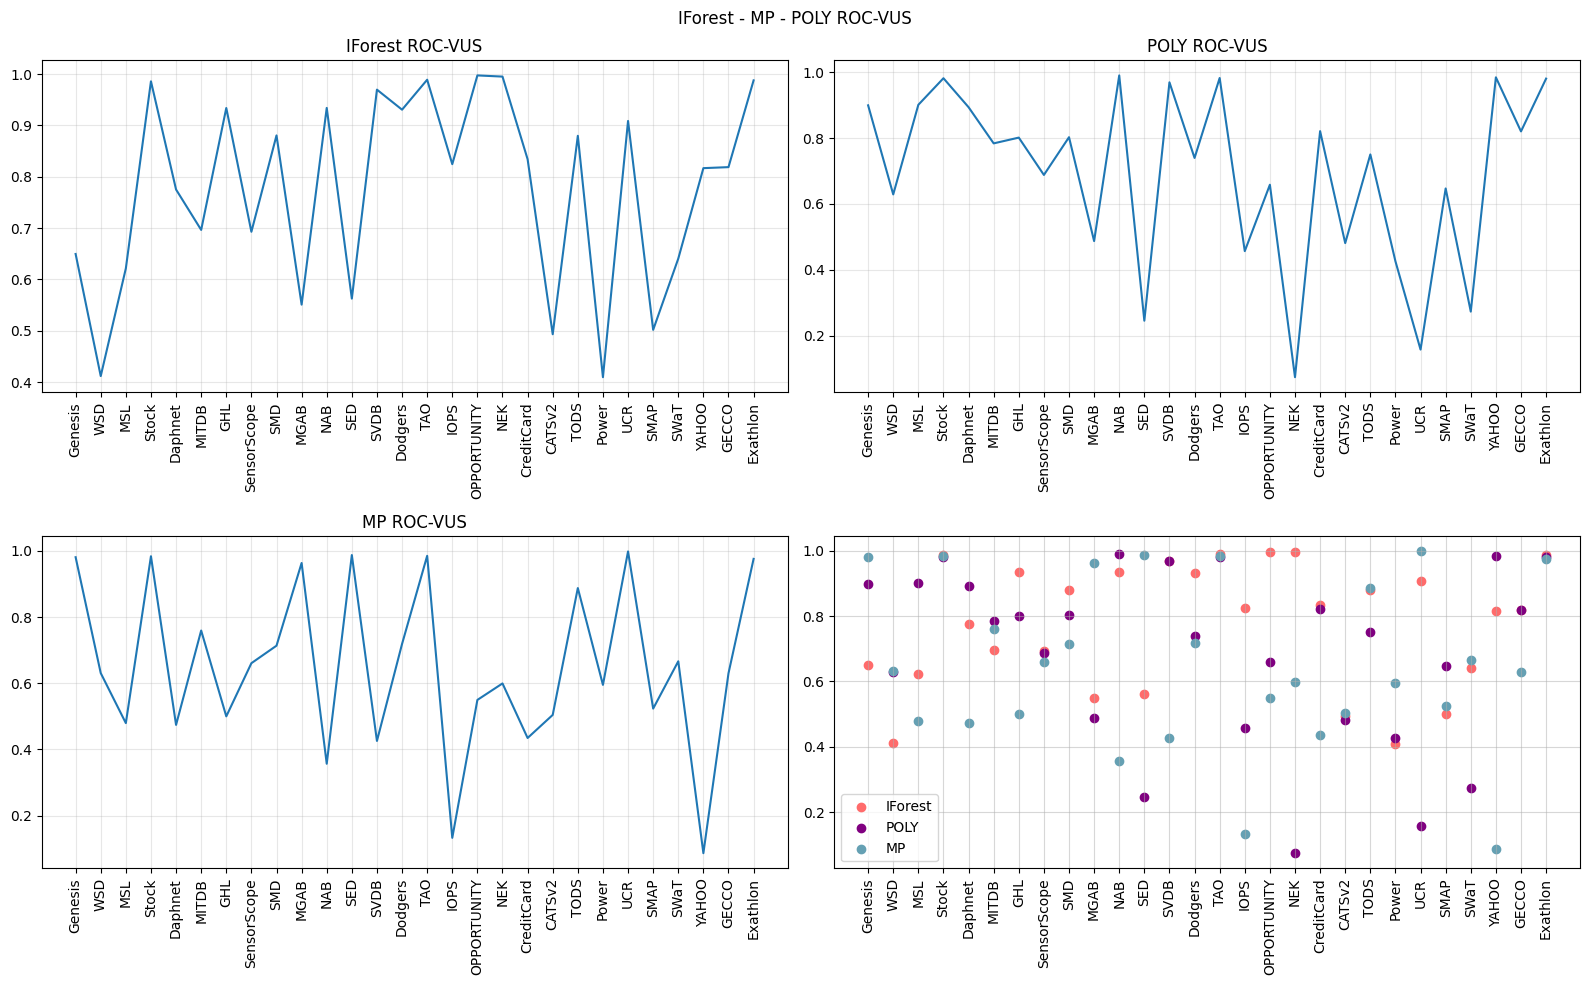
\includegraphics[width=1\linewidth]{Figures/v2_optuna-on_tsb-vus-compare.png}
    \caption{Αποτελέσματα χρήσης Optuna σε φθίνουσα σειρά.}
    \label{figure:tsad-vus-compare}
\end{figure}

Ιδιαίτερο ενδιαφέρον έχει όταν συγκρίνουμε όλα τα αποτελέσματα μεταξύ τους, δηλαδή του \emph{Auto-TSAD} και των αλγορίθμων του \emph{TSB-UAD}.Συγκριτκά τα αποτελέσματα του νικητήριου αλγορίθμου ανά dataset φαίνονται στον Πίνακα \ref{tab:winners}. Όπως φαίνεται και στο \ref{figure:vus-comparison-between-all}, θα περίμενε κανείς το \emph{Auto-TSAD}  να τα έχει πάει καλύτερα σε όλα τα dataset. Κάτι τέτοιο όμως δεν είναι αληθές και βλέπουμε ότι έχει καταφέρει να φέρει καλύτερα αποτελέσματα, μόνο στο $57,16\%$ των περιπτώσεων, γεγονός το οποίο είναι ιδιαίτερα χαμηλό αν αναλογιστεί κανείς το χρονικό κόστος. Η σημαντικότερη όμως παρατήρηση είναι, πως ακόμα και αν δεν κατάφερε να υπερτερήσει σε όλες τις περιπτώσεις, ήταν πολύ κοντά στην μέγιστη τιμή ανωμαλιών που ανιχτέυτηκε από τις άλλες τεχνικές.

\begin{table}
\centering
\caption{Νικητήριος Αλγόριθμος ανά Dataset}
\label{tab:winners}
\begin{tabular}{llc}
\toprule
 & Winner & Score \\
\midrule
Genesis & AutoTSAD & 0.9995 \\
WSD & AutoTSAD & 0.9987 \\
MSL & AutoTSAD & 0.9991 \\
Stock & IForest & 0.9860 \\
Daphnet & AutoTSAD & 0.9901 \\
MITDB & POLY & 0.7839 \\
GHL & AutoTSAD & 0.9982 \\
SensorScope & AutoTSAD & 0.7311 \\
SMD & AutoTSAD & 0.9922 \\
MGAB & AutoTSAD & 0.9994 \\
NAB & POLY & 0.9902 \\
SED & MP & 0.9873 \\
SVDB & AutoTSAD & 0.9806 \\
Dodgers & IForest & 0.9307 \\
TAO & IForest & 0.9891 \\
IOPS & AutoTSAD & 0.9856 \\
OPPORTUNITY & IForest & 0.9975 \\
NEK & IForest & 0.9953 \\
CreditCard & IForest & 0.8342 \\
CATSv2 & MP & 0.5044 \\
TODS & AutoTSAD & 0.9137 \\
Power & AutoTSAD & 0.9822 \\
UCR & AutoTSAD & 0.9988 \\
SMAP & AutoTSAD & 0.9986 \\
SWaT & AutoTSAD & 0.7014 \\
YAHOO & POLY & 0.9844 \\
GECCO & AutoTSAD & 0.9911 \\
Exathlon & IForest & 0.9879 \\
\bottomrule
\end{tabular}
\end{table}

\begin{figure}[h]
    \centering
    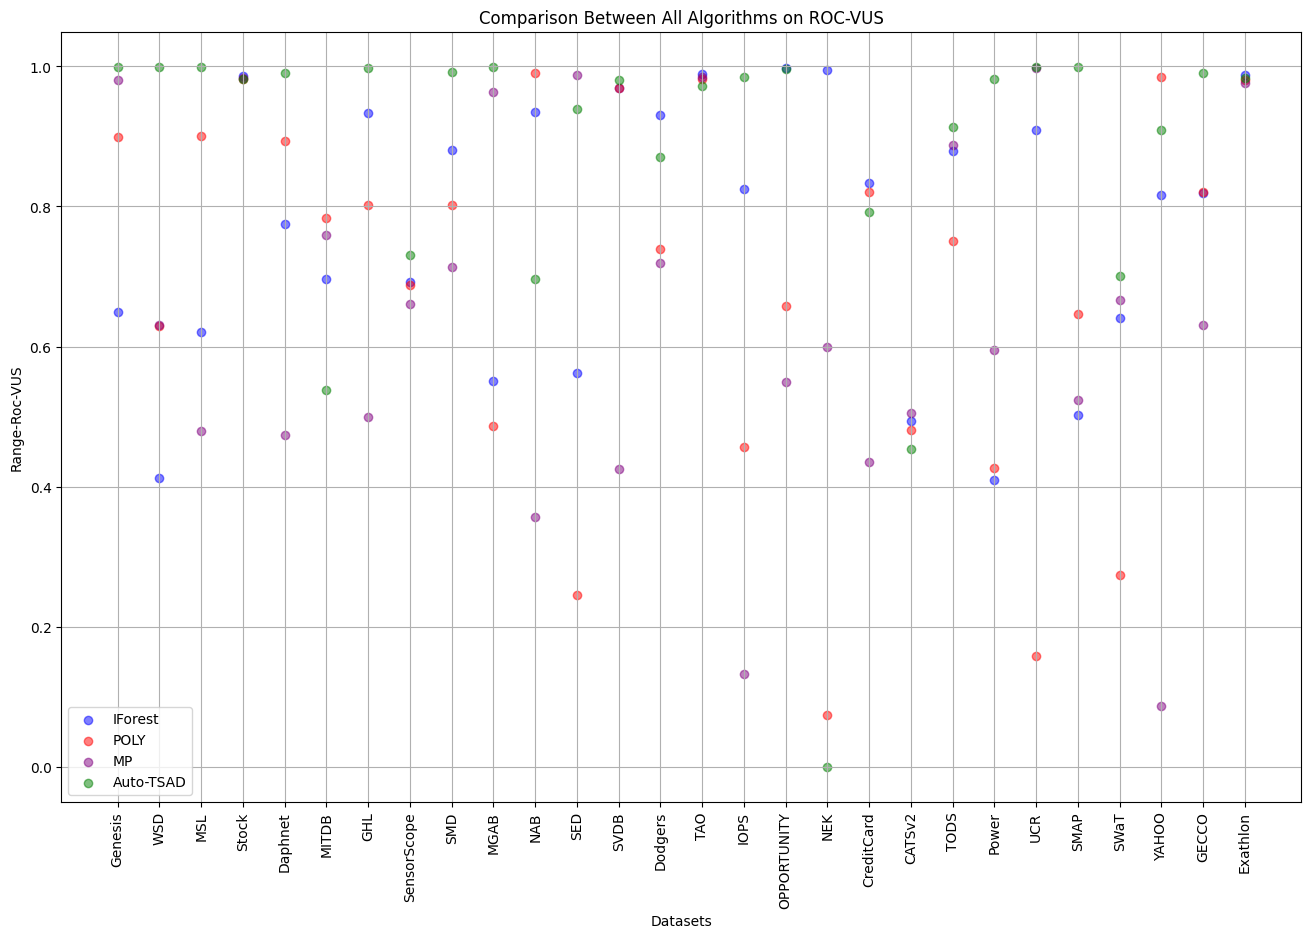
\includegraphics[width=1\linewidth]{Figures/vus-comparison-between-all.png}
    \caption{Σύγκριση μεταξύ όλων των τεχνικών.}
    \label{figure:vus-comparison-between-all}
\end{figure}

Πιο συγκερκιμένα και όπως φαίνεται και στο boxplot του σχήματος \ref{figure:more-comparisons}, το \emph{Auto-TSAD} έχει πολύ πιο σταθερή απόδοση σε σχέση με τους υπόλοιπους αλγορίθμους. Η διάμεσός του, η οποία δεν φαίνεται καθαρά, αγγίζει σχεδόν το $1.0$ και το κουτί του, είναι εξαιρετικά συμπιεσμένο προς τα πάνω. Ακολουθεί ο αλγόριθμος \emph{IForest} με καλύτερα αποτελέσματα από τους άλλους, ενώ ο \emph{POLY} και ο \emph{MP} έχουν σχεδόν παρόμοια συμπεριφορά.
Το barchart του σχήματος \ref{figure:more-comparisons} μας δείχνει ξεκάθαρα πως το \emph{Auto-TSAD} κυριαρχεί έναντι των άλλων μεθόδων με 16 νίκες, έναντι του \emph{IForest} με 8 νίκες και των \emph{POLY} και \emph{MP} με 3 και 2 νίκες αντιστοίχως.
Στο 3ο διάγραμμα του σχήματος \ref{figure:more-comparisons}, όποια κουκίδα βρίσκεται κάτω και δεξιά από την γραμμή $y=x$, σημαίνει ότι το \emph{Auto-TSAD} ξεπέρασε τον αντίστοιχο αλγόριθμο. Παρατηρήτε μία συγκέντρωση κουκκίδων, στην τέρμα δεξιά πλευρά, γεγονός το οποίο μας δείχνει πως όταν το \emph{Auto-TSAD} κατάφερε να πιάσει σχεδόν $100\%$ των ανωμαλιών, οι άλλοι αλγόριθμοι αποτύγχαναν αρκετές φορές. 

\begin{figure}[h]
    \centering
    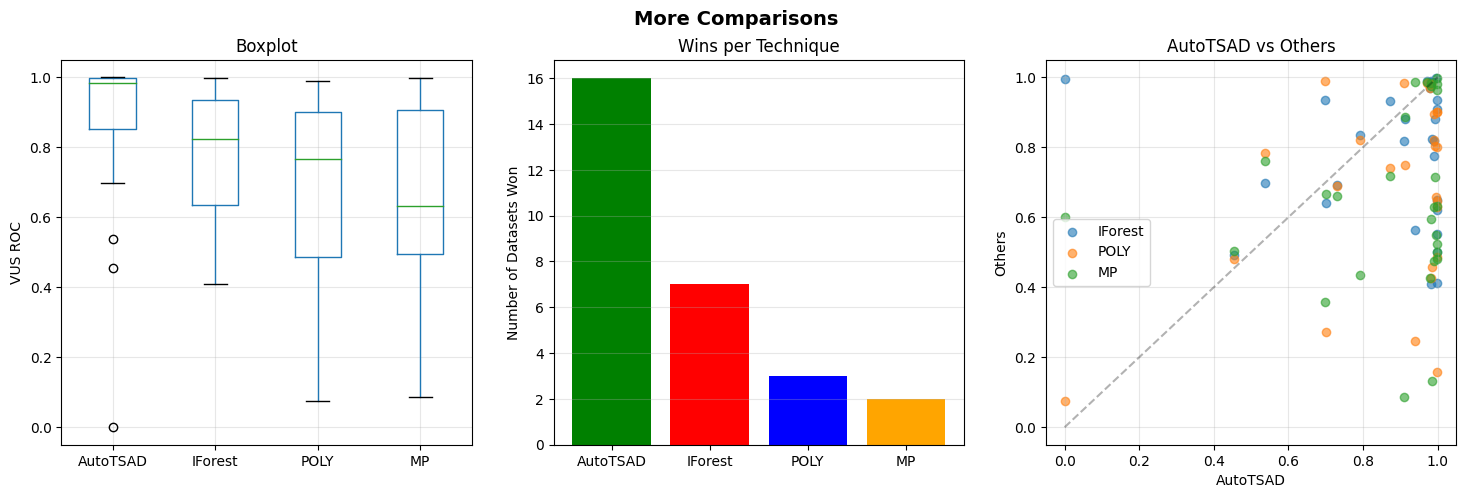
\includegraphics[width=1\linewidth]{Figures/v2_optuna-on_more_comparisons.png}
    \caption{Σύγκριση μεταξύ όλων των τεχνικών.}
    \label{figure:more-comparisons}
\end{figure}

Φτάνουμε λοιπόν στο συμπέρασμα πως υπάρχει ένα ξεκάθαρο αντιστάθισμα μεταξύ υπολογιστικού κόστους και ακρίβειας. Αν και η εκτέλεση μεμονωμένων αλγόριθμων απαιτεί μόνο μερικά δευτερόλεπτα με προκαθορισμένες υπερπαραμέτρους, η απόδοσή τους είναι εξαιρετικά ασταθής. Σε αντίθεση, οι τεχνικές βελτιστοποίησης του \emph{Auto-TSAD} αν και εκτοξεύουν το χρόνο εκτέλεσης σε τάξης αρκετών ωρών ή ακόμα και ημερών, εξασφαλίζουν σταθερότητα και ανωτερότητα στην εύρεση ενωμαλιών, εκτός μεμονωμένων περιπτώσεων.

\subsubsection{Συγκριτικά αποτελέσματα με Optuna-OFF}
Όπως έχουμε αναφέρει και στην αρχή του κεφαλαίου, χωρίς την μηχανή βελτιστοποίησης \emph{Optuna}, το \emph{Auto-TSAD} μπόρεσε να υπολογίσει αποτελέσματα μόνο στο $31,2\%$ των περιπτώσεων, ποσοστό αρκετά χαμηλό .
Στο σχήμα \ref{figure:roc-vus_optuna_off_v2} παρατηρούμε ότι οι τιμές της ROC-VUS διαφέρουν αρκετά σχετικά με το αν συμπεριλάβουμε τις αποτυχημένες προσπάθειες ή όχι. Συγκεκριμένα:
\begin{itemize}
    \item \strong{Με} συμπερίληψη των αποτυχημένων προσπαθειών, βλέπουμε ότι οι τιμές της ROV-VUS επειρεάζονται αρκετά από τις αποτυχίες και περιορίζονται στο διάστημα $[0,0.4]$. Επίσης η διάμεσος είναι $0.33$ και η τυπική απόκληση $0.41$.
    \item \strong{Χωρίς} συμπερίληψη αποτυχημένων προσπαθειών, η εικόνα αλλάζει δραματικά, η ελάχιστη τιμή είναι περίπου $0.42$, η μέγιστη αγγίζει το απόλυτο, ενώ υπάρχει μία συγκέντρωση τιμών στο διάστημα $[0.73, 0.96]$. Η διάμεσος είναι $0.84$ ενώ η τυπική απόκλιση είναι $0.11$.   
\end{itemize}
Παρατηρούμε λοιπόν, πως υπάρχει σημαντική διαφορά των αποτελεσμάτων, αν δεν συμπεριλάβουμε τα αποτελέσματα των αποτυχημένων προσπαθειών. 

\begin{figure}[h]
    \centering
    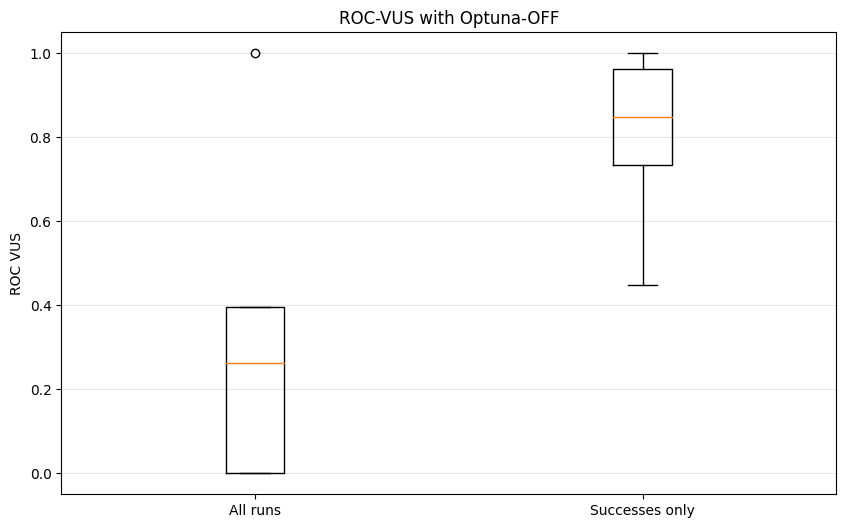
\includegraphics[width=0.8\linewidth]{Figures/roc-vus_optuna_off_v2.png}
    \caption{Αποτελέσματα Auto-TSAD με Optuna-OFF στο v2\_public dataset.}
    \label{figure:roc-vus_optuna_off_v2}
\end{figure}

Στο σχήμα \ref{figure:comparison_Between_Auto-TSAD_WO_Optuna_and_TSB-UAD_algorithms}, στο οποίο συγκρίνουμε την απόδοση του \emph{Auto-TSAD} χωρίς \emph{Optuna} με τους αλγορίθμους το \emph{TSB-UAD}, βλέπουμε πως, όταν ο \emph{Auto-TSAD} καταφέρνει να δώσει αποτέλεσμα, είναι αρκετά πιο αποτελεσματικούς από τους υπόλοιπους αλγορίθμους. Αν αντιθέτως συγκρίνουμε τα στατιστικά του συνυπολογίζοντας και τις αποτυχίες του, τότε οι απλοί αλγόριθμοι υπερτερούν αρκετά. Το μεγάλο πλεονέκτημα των αλγορίθμων του \emph{TSB-UAD}, είναι πως πάντα θα καταφέρουν να υπολογίσουν ένα μέρος των ανωμαλιών της χρονοσειράς που εξετάζουν, ακόμα και αν το αποτέλεσμα τους δεν είναι ικανοποιητικό. 
\begin{figure}[h]
    \centering
    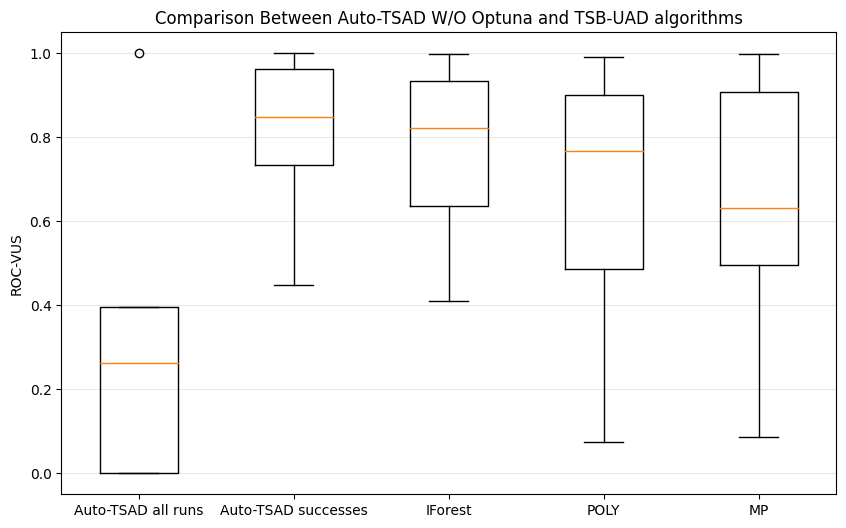
\includegraphics[width=0.8\linewidth]{Figures/Comparison_Between_Auto-TSAD_WO_Optuna_and_TSB-UAD_algorithms.png}
    \caption{Σύγκριση αποτελεσμάτων μεταξύ Auto-TSAD χωρίς Optuna και TSB-UAD.}
    \label{figure:comparison_Between_Auto-TSAD_WO_Optuna_and_TSB-UAD_algorithms}
\end{figure}

\textcolor{red}{ΕΡΩΤΗΜΑ ΠΡΟΣ Κ.ΓΟΥΝΑΡΗ. ΑΝ ΘΕΛΕΤΕ ΜΠΟΡΩ ΚΑΙ ΕΔΩ ΝΑ ΚΑΝΩ ΑΝΑΛΥΣΗ ΑΝΑ DATASET, ΚΑΙ ΟΧΙ ΣΥΓΚΕΝΤΡΩΤΙΚΑ.}
\section{Artificial Dataset}
\textcolor{red}{ΠΡΟΣ Κ.ΓΟΥΝΑΡΗ. ΕΔΩ ΘΑ ΕΧΩ ΤΗΝ ΙΔΙΑ ΑΝΑΛΥΣΗ ΟΠΩΣ ΣΤΟ PUBLIC DATASET, ΑΠΛΑ ΕΠΕΙΔΗ ΤO ARTIFICIAL ΔΕΝ ΧΩΡΊΖΕΙ ΣΕ ΔΙΑΦΟΡΕΤΙΚΟΥ ΤΥΠΟΥ ΔΕΔΟΜΕΝΩΝ Η ΑΝΑΛΥΣΗ ΘΑ ΕΙΝΑΙ ΠΙΟ ΣΥΝΤΟΜΗ}
\section{ΚΕΡΔΟΣ ΑΝΑ ΧΡΟΝΟ}
\textcolor{red}{ΠΡΟΣ Κ.ΓΟΥΝΑΡΗ. ΕΔΩ ΘΑ ΒΑΛΩ ΑΥΤΟ ΠΟΥ ΜΕ ΕΙΠΑΤΕ, ΟΠΟΥ ΘΑ ΠΟΣΟ ΚΕΡΔΙΖΩ ΣΤΗΝ ROC VUS // ΜΟΝΑΔΕΣ ΧΡΟΝΟΥ}